%%%%%%%%%%%%%%%%%%%%%%%%%%%%%%%%%%%%%%%%%
% Short Sectioned Assignment
% LaTeX Template
% Version 1.0 (5/5/12)
%
% This template has been downloaded from:
% http://www.LaTeXTemplates.com
%
% Original author:
% Frits Wenneker (http://www.howtotex.com)
%
% License:
% CC BY-NC-SA 3.0 (http://creativecommons.org/licenses/by-nc-sa/3.0/)
%
%%%%%%%%%%%%%%%%%%%%%%%%%%%%%%%%%%%%%%%%%

%----------------------------------------------------------------------------------------
%	PACKAGES AND OTHER DOCUMENT CONFIGURATIONS
%----------------------------------------------------------------------------------------

\documentclass[paper=a4, fontsize=11pt]{scrartcl} % A4 paper and 11pt font size
\usepackage{graphicx}
\usepackage{wrapfig}
\usepackage[T1]{fontenc} % Use 8-bit encoding that has 256 glyphs
%\usepackage{fourier} % Use the Adobe Utopia font for the document - comment this line to return to the LaTeX default
\usepackage[english]{babel} % English language/hyphenation
\usepackage{amsmath,amsfonts,amsthm} % Math packages
\usepackage{sectsty} % Allows customizing section commands
\usepackage{changes}
\usepackage{amsmath,mathtools}
\usepackage{cancel}
\setdeletedmarkup{\cancel{#1}}

\allsectionsfont{\centering \normalfont\scshape} % Make all sections centered, the default font and small caps

\usepackage{fancyhdr} % Custom headers and footers
\pagestyle{fancyplain} % Makes all pages in the document conform to the custom headers and footers
\fancyhead{} % No page header - if you want one, create it in the same way as the footers below
\fancyfoot[L]{} % Empty left footer
\fancyfoot[C]{} % Empty center footer
\fancyfoot[R]{\thepage} % Page numbering for right footer
\renewcommand{\headrulewidth}{0pt} % Remove header underlines
\renewcommand{\footrulewidth}{0pt} % Remove footer underlines
\setlength{\headheight}{13.6pt} % Customize the height of the header

\numberwithin{equation}{section} % Number equations within sections (i.e. 1.1, 1.2, 2.1, 2.2 instead of 1, 2, 3, 4)
\numberwithin{figure}{section} % Number figures within sections (i.e. 1.1, 1.2, 2.1, 2.2 instead of 1, 2, 3, 4)
\numberwithin{table}{section} % Number tables within sections (i.e. 1.1, 1.2, 2.1, 2.2 instead of 1, 2, 3, 4)
\newtheorem{theorem}{Theorem}
 \newtheorem{definition}{Definition}
 \newtheorem{example}{Example}
  \newtheorem{exercise}{Exercise}
  \numberwithin{exercise}{section}
  
\setlength\parindent{0pt} % Removes all indentation from paragraphs - comment this line for an assignment with lots of text

%----------------------------------------------------------------------------------------
%	TITLE SECTION
%----------------------------------------------------------------------------------------

\newcommand{\horrule}[1]{\rule{\linewidth}{#1}} % Create horizontal rule command with 1 argument of height

\title{	
\normalfont \normalsize 
%
\horrule{0.5pt} \\[0.4cm] % Thin top horizontal rule
\huge Chapter I: Fundamentals   \\ % The assignment title
\horrule{2pt} \\[0.5cm] % Thick bottom horizontal rule
}
\date{}
\author{Aili Shao} 


\begin{document}

\maketitle % Print the title

%----------------------------------------------------------------------------------------
%	PROBLEM 1
%----------------------------------------------------------------------------------------

\section{ Lecture 1 Matrix- Vector Multiplication (21/04/2018)}

\begin{exercise} 
(a)
Row operation $\to$ Multiply a matrix on the left of $B$;

Column operation $\to$ Multiply a matrix on the right of $B$.
\begin{enumerate}
\item double column  $1$ : Multiply on the right of $B$ by
$ R_1=\begin{bmatrix}
2&  0 & 0 & 0 \\
0 & 1 & 0 & 0 \\
0 & 0 & 1 & 0 \\
0 & 0 & 0 & 1 \\
\end{bmatrix}.$
\item halve row $3$: Multiply on the left of $B$ by 
$ L_1=\begin{bmatrix}
1& 0 & 0 & 0 \\
0 & 1 &  0& 0 \\
0 & 0 & 1/2 & 0 \\
0 & 0 & 0 & 1\\
\end{bmatrix}.$
\item add row $3$ to row $1$:
Multiply on the left of $B$ by 
$ L_2=\begin{bmatrix}
1& 0 &1  & 0 \\
0 & 1 & 0& 0 \\
0 & 0 & 1 & 0 \\
0 & 0 &  0& 1\\
\end{bmatrix}.$
\item interchange columns $1$ and $4$: Multiply on the right of $B$ by 
$ R_2=\begin{bmatrix}
0& 0 & 0 & 1 \\
0 & 1 &  0& 0 \\
0 & 0 & 1 & 0 \\
1 & 0 & 0 & 0\\
\end{bmatrix}.$
\item subtract row $2$ from each of the other rows:
Multiply on the left of $B$ by 
$ L_3=\begin{bmatrix}
1& -1 & 0 & 0 \\
0 & -1 &  0& 0 \\
0 & -1 & 1 & 0 \\
0 & -1 & 0 & 1\\
\end{bmatrix}.$
\item  replace column $4$ by column $3$:  Multiply on the right of $B$ by 
$ R_3=\begin{bmatrix}
1& 0 & 0 & 0\\
0 & 1 &  0& 0 \\
0 & 0 & 1 & 1 \\
0 & 0 & 0 & 0\\
\end{bmatrix}.$
\item  delete column $1$ : 
Multiply on the right of $B$ by 
$ R_4=\begin{bmatrix}
0 & 0 & 0\\
1 &  0& 0 \\
 0 & 1 & 0\\
 0 & 0& 1\\
\end{bmatrix}.$
\end{enumerate}
Thus the resulting matrix is 

$$ \begin{bmatrix}
1& -1& 0 & 0 \\
0 & -1&  0& 0 \\
0 & -1 & 1 & 0 \\
0 & -1 & 0 & 1\\
\end{bmatrix}\begin{bmatrix}
1& 0 &1  & 0 \\
0 & 1 & 0& 0 \\
0 & 0 & 1 & 0 \\
0 & 0 &  0& 1\\
\end{bmatrix}\begin{bmatrix}
1& 0 & 0 & 0 \\
0 & 1 &  0& 0 \\
0 & 0 & 1/2 & 0 \\
0 & 0 & 0 & 1\\
\end{bmatrix}B\begin{bmatrix}
2&  0 & 0 & 0 \\
0 & 1 & 0 & 0 \\
0 & 0 & 1 & 0 \\
0 & 0 & 0 & 1 \\
\end{bmatrix}\begin{bmatrix}
0& 0 & 0 & 1 \\
0 & 1 &  0& 0 \\
0 & 0 & 1& 0 \\
1 & 0 & 0 & 0\\
\end{bmatrix}\begin{bmatrix}
1& 0 & 0 & 0\\
0 & 1 &  0& 0 \\
0 & 0 & 1& 1 \\
0 & 0 & 0& 0\\
\end{bmatrix}\begin{bmatrix}
0 & 0 & 0\\
1 &  0& 0 \\
 0 & 1 & 0\\
 0 & 0& 1\\
\end{bmatrix}$$
(b)

$$A=L_3L_2L_1= \begin{bmatrix}
1& -1& 0 & 0 \\
0 & -1&  0& 0 \\
0 & -1 & 1 & 0 \\
0 & -1 & 0 & 1\\
\end{bmatrix}\begin{bmatrix}
1& 0 &1  & 0 \\
0 & 1 & 0& 0 \\
0 & 0 & 1 & 0 \\
0 & 0 &  0& 1\\
\end{bmatrix}\begin{bmatrix}
1& 0 & 0 & 0 \\
0 & 1 &  0& 0 \\
0 & 0 & 1/2 & 0 \\
0 & 0 & 0 & 1\\
\end{bmatrix}=\begin{bmatrix}
1& 0 & 0 & 0 \\
0 & 1 &  0& 0 \\
0 & 0 & 1/2 & 0 \\
0 & 0 & 0 & 1\\
\end{bmatrix}
=\begin{bmatrix}
 0 &-1& 1/2& 0\\
 0 &-1& 0& 0\\
  0 &-1 &1/2& 0\\
  0& -1 & 0& 1\\\end{bmatrix}$$
 
 $$C=R_1R_2R_3R_4=\begin{bmatrix}
2&  0 & 0 & 0 \\
0 & 1 & 0 & 0 \\
0 & 0 & 1 & 0 \\
0 & 0 & 0 & 1 \\
\end{bmatrix}\begin{bmatrix}
0& 0 & 0 & 1 \\
0 & 1 &  0& 0 \\
0 & 0 & 1& 0 \\
1 & 0 & 0 & 0\\
\end{bmatrix}\begin{bmatrix}
1& 0 & 0 & 0\\
0 & 1 &  0& 0 \\
0 & 0 & 1& 1 \\
0 & 0 & 0& 0\\
\end{bmatrix}\begin{bmatrix}
0 & 0 & 0\\
1 &  0& 0 \\
 0 & 1 & 0\\
 0 & 0& 1\\
\end{bmatrix}=\begin{bmatrix}
0 & 0 & 0\\
1 &  0& 0 \\
 0 & 1 & 1\\
 0 & 0& 0\\
\end{bmatrix}.$$
\end{exercise}
\begin{exercise}
(a) We know that 
$$f_1=k_{12}(x_2-x_1-l_{12});$$
$$f_2=k_{23}(x_3-x_2-l_{23});$$
$$f_3=k_{34}(x_4-x_3-l_{34});$$
$$f_4=0.$$
By writing the above linear system as matrix-vector multiplication we have
$$\begin{bmatrix}
f_1\\
f_2\\
f_3\\
f_4
\end{bmatrix}=\begin{bmatrix}
- k_{12} & k_{12} & 0 & 0 \\ 0 & -k_{23}& k_{23} & 0 \\ 0 & 0 & -k_{34} & k_{34} \\ 0 & 0& 0& 0\\
\end{bmatrix}\begin{bmatrix}
x_1\\x_2\\x_3\\x_4
\end{bmatrix} -\begin{bmatrix}
k_{12}l_{12}\\k_{23}l_{23}\\k_{34}l_{34}\\ 0
\end{bmatrix}.$$
(b) $K=\begin{bmatrix}
- k_{12} & k_{12} & 0 & 0 \\ 0 & -k_{23}& k_{23} & 0 \\ 0 & 0 & -k_{34} & k_{34} \\ 0 & 0& 0& 0\\
\end{bmatrix}.$

The entries of $K$ are spring constants. By Hook's law, we know that  force=spring constant $\times$ displacement.
Thus, the entries of $K$ are $\frac{\mathbf{force}}{\mathbf{displacement}}=\frac{ma}{d}=\frac{\mathbf{mass}}{\mathbf{time}^2}.$

(c) The dimensions of $\det(K)=\left( \frac{\mathbf{mass}}{\mathbf{time}^2 }  \right)^4.$

(d) Since the dimensions of entry of $K$ only involves time and mass. The SI unit of time is second while the SI unit of mass is kilogram. $1 \mathbf{kg}=1000 \mathbf{g}$. Thus $K'=1000 K$  and $\det(K')=1000^4 \det(K)$.
\end{exercise}

\begin{exercise}
We first write  $R$ as
$$R=\begin{bmatrix}
r_{1,1} & r_{1,2} & r_{1,3}&\dots & r_{1,m} \\
0 & r_{2,2} &  r_{2,3} &\dots  & r_{2,m}\\
0& 0 &  r_{3,3} &\dots & r_{3,m} \\
\vdots & \ddots & \\
0 & 0 & 0 &\dots & r_{m,m} \\
\end{bmatrix}= \Bigg[ r_1 \Big | r_2  \Big | \cdots  \Big | r_m\Bigg]$$.

Let $e_j$ denote the canonical unit vector with $1$ in the $j$th entry.
Then 
$$e_j=\sum_{i=1}^m z_{ij}r_i.$$
In particular $$e_1=\begin{bmatrix}
1\\
0\\
\vdots \\
0\end{bmatrix}=z_{1,1}\begin{bmatrix}
r_{1,1}\\
0\\
\vdots \\
0\end{bmatrix}+z_{2,1}\begin{bmatrix}
r_{1,2}\\
r_{2,2}\\
\vdots \\
0\end{bmatrix}+z_{3,1}\begin{bmatrix}
r_{1,3}\\
r_{2,3}\\
\vdots \\
0\end{bmatrix} +\cdots+z_{m,1}\begin{bmatrix}
r_{1,m}\\
r_{2,m}\\
\vdots \\
r_{m,m}\end{bmatrix}.$$

That is $z_{m,1} r_{m,m}=0$ which implies $z_{m,1}=0.$  This means that $e_1$ is spanned by $\{ r_1, r_2,\cdots r_{m-1}\}$ only. More precisely,
$$e_1=\begin{bmatrix}
1\\
0\\
\vdots \\
0\end{bmatrix}=z_{1,1}\begin{bmatrix}
r_{1,1}\\
0\\
\vdots \\
0\end{bmatrix}+z_{2,1}\begin{bmatrix}
r_{1,2}\\
r_{2,2}\\
\vdots \\
0\end{bmatrix}+z_{3,1}\begin{bmatrix}
r_{1,3}\\
r_{2,3}\\
\vdots \\
0\end{bmatrix} +\cdots+z_{m-1,1}\begin{bmatrix}
r_{1,m-1}\\
r_{2,m-1}\\
\vdots \\
r_{m-1,m-1}\end{bmatrix}.
$$
Then we can get $z_{m-1,1}r_{m-1,m-1}=0$, which implies that $z_{m-1,1}=0.$
Similarly, we can show that $z_{m-2, 1}=z_{m-2,1}=\cdots=z_{2,1}=0.$

Now we consider a general canonical unit vector 
$$e_j=\begin{bmatrix}
0\\
\vdots \\
j\\
\vdots\end{bmatrix}=z_{1j}\begin{bmatrix}
r_11\\
0\\
\vdots \\
0\end{bmatrix}+z_{2j}\begin{bmatrix}
r_{12}\\
r_{22}\\
\vdots \\
0\end{bmatrix}+z_{3j}\begin{bmatrix}
r_{13}\\
r_{23}\\
\vdots \\
0\end{bmatrix} +\cdots+z_{mj}\begin{bmatrix}
r_{1m}\\
r_{2m}\\
\vdots \\
r_{mm}\end{bmatrix}.$$

Thus, $z_{m,j}=z_{m-1,j}=\cdots z_{j+1,j}=0$ for every $j=1,2,\cdots, m.$ That is, $Z$ is also an upper-triangular matrix.

Note that $e_j=R z_j$, so we have $I=RZ.$ That is, $Z=R^{-1}$. This completes the proof.
\end{exercise}

\begin{exercise}
(a) We can write 
$$\sum_{j=1}^8 c_j f_j(i) =d_i \mbox { for } i=1,2,\cdots 8$$
as matrix-vector multiplication:
$$d=Fc$$
where $d=\begin{bmatrix}
d_1\\d_2\\
\vdots \\
d_8
\end{bmatrix},
 c=\begin{bmatrix}
 c_1\\c_2\\
 \vdots \\
c_8
\end{bmatrix}$ while $F$ is a $8\times 8$ square matrix with the $i,j$th entry defined by $F_{ij}:=f_j(i)$.

Since for each $d\in\mathbb{C}^8$, we can find $c\in \mathbb{C}^8$ such that $d=Fc$, the range of $A$ is $\mathbb{C}^8$. By the equivalent theorem(Theorem 1.3 in the book), we know that $\mathbf{rank}\left(F\right)=8$. This implies that $F$ has an inverse, and thus $d$ determines $c$ uniquely if we multiply the matrix-vector multiplication expression $d=Fc$ by $F^{-1}$ on both sides.

(b) By definition, we have $Ad=c$. That is, $A=F^{-1}$. Thus $A^{-1}=F$.  The $ij$ entry of $A^{-1}$ is simply the $ij$th entry of $F$, that is, $f_j(i)$.

\end{exercise}
\section{ Lecture 2  Orthogonal Vectors and Matrices (24/04/2018)}
\begin{exercise}
If $A$ is upper-triangular, then $A^{-1}$ is upper-triangular (by Exercise 1.3). Since $A$ is also unitary, we know that $A^{\star}=A^{-1}$ is upper triangular . However, $A^{\star}$,  as a transpose of an upper-triangular matrix, should be lower-triangular. Thus, $A^{-1}$ must be diagonal.  This implies that $A$ is diagonal.  The argument is the same when $A$ is lower- triangular.
\end{exercise}
\begin{exercise}
(a) $$\|x_1+x_2\|^2=x_1^2+x_2^2+\deleted{2 x_1\cdot x_2}=x_1^2+x_2^2$$
since $x_1$ is orthogonal to $x_2$.

(b) Assume the equality holds for sum up to $n-1$, that is 
$$\|\sum_{i=1}^{n-1} x_i\|^2=\sum_{i=1}^{n-1} \|x_i\|^2.$$
Then 
\begin{align*}
\|\sum_{i=1}^{n} x_i\|^2=&\|\sum_{i=1}^{n-1} x_i +x_n\|^2\\
{}=&\|\sum_{i=1}^{n-1} x_i \|^2+x_n^2+\deleted{2 \sum_{i=1}^{n-1} x_n\cdot x_i}\\
{}=&\|\sum_{i=1}^{n} x_i \|^2
\end{align*}
as $x_n$ is orthogonal to $x_i$ for $i=1,2,\cdots,n-1.$
\end{exercise}
\begin{exercise}

(a)Assume that $\lambda$ is an eigenvalue of $A$, then there exists non-zero $x$ such that $Ax=\lambda x$. Then, using that $A^{\star}=A.$
$${x^{\star} }A x={x^{\star}}(Ax)={x^{\star}}(\lambda x)=\lambda (x^{\star} \cdot x),$$
$${x^{\star}}A x=(A{x})^{\star}x=({\lambda}{x} )^{\star} x={\lambda}^{\star} ({x^\star} \cdot x).$$
 Since $x\neq 0$, $({x^{\star}},x)>0.$ Thus, ${\lambda^{\star}}=\lambda$. That is, $\lambda\in\mathbb{R}.$
 
 (b) Assume that $Ay=\lambda y, Ax=\mu x$, then using $A^\star=A$,
 
 $${x^\star} Ay={x^{\star}}(Ay)={x^\star} \lambda y=\lambda {x^\star} y=\lambda (x\cdot y),$$
  $$x^{\star} Ay= (Ax)^{\star} y=(\mu x)^{\star} y=\mu ^{\star}  x^{\star}  y =\mu  (x\cdot y).$$
 The last equality follows from the fact that all eigenvalues are real.
 Since $\lambda\neq \mu,$ $x\cdot y=0$. That is, $x$ is orthogonal to $y$.
\end{exercise}
\begin{exercise}
The eigenvalues of a unitary matrix has modulus $1$.
Using $A^{-1}=A^{\star}$, we have
 $$x^{\star}x=x^{\star} A^{-1} Ax=(x^{\star} A^{\star})( Ax)=(\lambda^{\star} x^{\star} (\lambda x)=|\lambda|^2  x^{\star} x.$$

 Thus $|\lambda|=1.$
\end{exercise}
\begin{exercise}
(a) Similar to  the proof in Exercise 2.3 (a), we have $\lambda=-\lambda^{\star}$ in this case. This implies that the eigenvalues of $S$ are pure imaginary. 

(b) If there exists non-zero $x$ such that  $(I-S)x=0.$ Then 
$x=Sx.$  
$$x^{\star} x=(Sx)^{\star} x=x^{\star} S^{\star} x=x^{\star} (-S)x=-x^{\star} x.$$

Thus $x\equiv 0$. That is, $\mathrm{Null}(I-S)=\{0\}$, so $I-S$ is non-singular.

(c) 
$$Q^{\star}=(I+S)^{\star}((I-S)^{-1})^{\star}=(S^\star+I)[(I-S)^{\star}]^{-1}=(I-S)(I+S)^{-1}=Q^{-1}.$$
\end{exercise}
\begin{exercise}

If $u\equiv 0$, then it is trivial. Now assume that $u\neq 0.$

If $A$ is non-singular, we can find out $A^{-1}$.  We write 
$$A^{-1}=\left[ x_1, x_2, \cdots, x_m \right]$$ where $x_i$ represents the $i$th column of $A^{-1}$.
Then 
\begin{align*}
AA^{-1}=& (I+uv^{\star})\left[ x_1, x_2, \cdots, x_m \right]\\
{}=& \left[1+uv^{\star}x_1, \cdots, x_m+uv^{\star} x_m\right]\\
{}=&I\\
{}=&\left[ e_1, e_2, \cdots, e_m\right]
\end{align*}
This implies that $x_i+uv^{\star} x_i=e_i$ for each $1\leq i\leq m.$
Then we can write 
$$A^{-1}=\left[e_1-z_1u, e_2-z_2u, \cdots, e_m-z_m u\right]=I-uz^{\star}.$$
\begin{align*}
I=& AA^{-1}\\
{}=& (I+ u v^{\star})(I-uz^{\star})\\
{}=& I +uv^{\star}-uz^{\star} -uv^{\star} uz^{\star}\\
{}=&  I +uv^{\star}-uz^{\star} -(v^{\star} u)uz^{\star}\\
{}=& I.
\end{align*}
This means that 
$$uv^{\star}-uz^{\star} -(v^{\star} u)uz^{\star}
=0.$$
$$uz^{\star} (v^{\star} u+1)=uv^{\star}.$$
$$uz^{\star}=\frac{uv^{\star}}{v^{\star}u+1}.$$
This shows that 
$$z^{\star}=\frac{v^{\star}}{v^{\star}u+1}.$$
Thus, $A^{-1}=I-\frac{uv^{\star}}{v^{\star}u+1}=I+\alpha uv^{\star}$ where $\alpha=-\frac{1}{v^{\star}u+1}.$

Now we suppose that $A$ is singular, then there exists a non-zero $x$ such that $Ax=0$, that is $$(I+uv^{\star})x=0.$$
This implies that 

$$x=-uv^{\star}x.$$
$$x=-u(v^{\star}x)$$
where $v^\star x$ is a scalar.

This shows that $x=\beta u$ for some scaler $\beta$. If we plug $x=\beta u$ into $Ax=0,$ we get 
\begin{align*}
(I+uv^{\star}) \beta u =& \beta u+\beta u v^{\star} u\\
{}=& \beta u(1+v^{\star} u)\\
{}=&0.
\end{align*}
Since $\beta u\neq 0$, we must have $v^{\star}u=-1.$

If $A$ is singular, $\mathrm{null} (A)=\{\beta u \colon \beta\in \mathbb{C}\}.$



\end{exercise}
\begin{exercise}
Note that 
$$H_{k+1}^{-1}=\begin{bmatrix}
(2H_k)^{-1}  &   (2H_k)^{-1}\\
(2H_k)^{-1}  &  (-H_k)^{-1} +(2H_k)^{-1}\\
\end{bmatrix}=\frac{1}{2}\begin{bmatrix}
H_k^{-1}  &   H_k^{-1}\\
H_k^{-1}  & -H_k^{-1} \\
\end{bmatrix},$$

$$H_{k+1}^{T}=\begin{bmatrix}
H_k^{T}  &  H_k^{T} \\
H_k^{T}   &  -H_k^{T} \\
\end{bmatrix}=\frac{1}{2}\begin{bmatrix}
\alpha_k H_k^{-1}  &   \alpha_kH_k^{-1}\\
\alpha_kH_k^{-1}  & -\alpha_kH_k^{-1} \\
\end{bmatrix}=2\alpha_k H_{k+1}^{-1}.$$
By induction, the recursive description provides a Hadamard matrix for each $m=2^k$.
\end{exercise}
\section{Lecture 3 Norms (01/05/2018)}
\begin{exercise}
By definition,
$$\|x\|_{W}=\|Wx\|.$$
\begin{enumerate}
\item $\|x\|_{W}\geq 0,$ and $\|x\|_{W}=0$ only if $Wx=0$ which implies that $x=0$ since $W$ is non-singular.
\item $\|x+y\|_{W}=\|W(x+y)\|\leq \|Wx\|+\|Wy\|=\|x\|_{W}+\|y\|_{W}.$
\item $\|\alpha x\|_{W}=\|W(\alpha x)\|=\|\alpha Wx\|=|\alpha|\|Wx\|=|\alpha|\|x\|_{W}.$
\end{enumerate}
Thus $\|\cdot\|_{W}$ defines a vector norm for any arbitrary non-singular matrix $W$.
\end{exercise}
\begin{exercise}
By definition, we have
$\|A\|=\sup_{x \in\mathbb{C}^n,x\neq 0 } \frac{\|Ax\|}{\|x\|}$.
Since $\rho(A)$ is the largest absolute value $|\lambda|$ of an eigenvalue $\lambda$ of $A$. There exists a non-zero $y\in\mathbb{C}^n$, such that $Ay=\lambda y.$
That is, $\|Ay\|=|\lambda | \|y\|.$  Thus,
$$|\lambda |=\frac{\|Ay\|}{\|y\|} \leq \sup_{x \in\mathbb{C}^n,x\neq 0 } \frac{\|Ax\|}{\|x\|}=\|A\|.$$
\end{exercise}
\begin{exercise}
\begin{enumerate}

\item $\|x\|_{\infty} \leq \|x\|_2$ can be easily proved:
$$ \|x\|_2=\sqrt{\sum_{i=1}^m x_i^2} \geq |x_i| \mbox{ for  every }  1\leq i\leq n.$$

Take $x=e_1=(1,0,\cdots,0),$ then $\|x\|_{\infty} = \|x\|_2.$
\item  $\|x\|_{2} \leq \sqrt{m}\|x\|_{\infty}$ can be proved in the following way:
$$ \|x\|_2=\sqrt{\sum_{i=1}^m x_i^2} \leq  \sqrt{\sum_{i=1}^m \|x\|_{\infty}^2 }=\sqrt{m \|x\|_{\infty}^2 }=\sqrt{m}\|x\|_{\infty}.$$
Take $x=(1,1,\cdots,1)$. Then $\|x\|_2=\sqrt{\sum_{i=1}^m 1^2}=\sqrt{m}.$ $\sqrt{m}\|x\|_{\infty}=\sqrt{m}\cdot 1=\sqrt{m}.$

\item By part (1) and part (2), $\|A\|_{\infty}=\sup_{x\in\mathbb{C}^n\setminus\{ 0\}} \frac{\|Ax\|_{\infty}}{\|x\|_{\infty}}\leq \frac{\|Ax\|_2}{1/\sqrt{n}\|x\|_2}\leq \sqrt{n} \|A\|_2.$

Recall that $\|A\|_{\infty}$ is the maximum row sum while $\|A\|_2$ is the maximum absolute value of the singular value (eigenvalue for square matrix). 
Take $$A=\begin{bmatrix}
1 & 1\\
0 & \sqrt{2} \\
\end{bmatrix},$$ then $\|A\|_{\infty}=2, \|A\|_{2}=\sqrt{2}, \sqrt{n}=\sqrt{2},$ so the equality holds.
\item By part(1) and part (2),  $\|A\|_{2}=\sup_{x\in\mathbb{C}^n\setminus\{ 0\}} \frac{\|Ax\|_{2}}{\|x\|_{2}}\leq \frac{\sqrt{m} \|Ax\|_{\infty}}{ \|x\|_{\infty}}\leq \sqrt{m} \|A\|_{\infty}.$
Similar to (3), but we consider a rectangle matrix in this case. Take 
$$A=\begin{bmatrix}
1  & 0\\
\end{bmatrix},$$ then $\|A\|_2=1$ (the largest singular value of $A$), $\|A\|_{\infty}=1$ and $m=1,$ so 
$\|A\|_2=\sqrt{1} \|A\|_{\infty}.$
\end{enumerate}
\end{exercise}

\begin{exercise}
(a) Similar to the step 7 in Exercise 1.1, if we multiply on the RHS of $A$ by an identity matrix with $i$th column removed, the $i$th column of $A$ is deleted. If we multiply $A$ by an identity matrix with $j$th row removed on the LHS of $A$, the $j$th row of $A$ is deleted. We can multiply $A$ by such matrices to obtain $B$.

(b) We know that $\| AB\|_{p}\leq \|A\|_{p}\|B\|_{p}$ for any $m\times n$ matrix $A$, $n\times l$ matrix $B$ and for every $1\leq p\leq \infty.$ It is sufficient to show that $p$-norm of each matrix we used to multiply on the LHS and RHS of $A$ is less than or equal to $1$. This follows from direct computation.
\end{exercise}

\begin{exercise}
Since
$$ \frac{ \|Ex\|_{2}}{\|x\|_{2}}=\frac{\|uv^{\star} x\|_{2}}{\|x\|_{2}}= \frac{ \|u\|_2   |v^{\star}x|}{\|x\|_2} \leq \frac{ \|u\|_2  \|v\|_{2}\|x\|_{2}}{\|x\|_2}=\|u\|_2\|v\|_2 ,$$
$$\|E\|_2=\sup_{x\in\mathbb{C}^n\setminus \{0\}}\frac{ \|Ex\|_{2}}{\|x\|_{2}}\leq \|u\|_2\|v\|_2.$$
The equality is achieved if we take $x=v$. Thus,
$$\|E\|_2=\|u\|_2\|v\|_2.$$

Note that $E_{ij}=u_i v_j$, thus
$$\|E\|_{F}=\sqrt{\sum_{i=1}^m\sum_{j=1}^n |E_{ij}|^2 }=\sqrt{\sum_{i=1}^m\sum_{j=1}^n |u_i|^2 |v_j|^2}=\sqrt{\sum_{i=1}^m |u_i|^2}\sqrt{\sum_{j=1}^n |v_j|^2}=\|u|_{F}\|v\|_{F}.$$
\end{exercise}

\begin{exercise}

(a)
\begin{enumerate}
\item By definition $\|x\|^{'}=\sup_{\|y\|=1}|y^{\star}x|\geq 0$ and $\|x\|^{'}=0$ only if  $x=0.$
\item  $\|x+z\|^{'} =\sup_{\|y\|=1}|y^{\star}(x+z)|\leq\sup_{\|y\|=1}(|y^{\star}x| +|y^{\star}z|)=\|x\|^{'}+\|z\|^{'}.$
\item $\|\alpha x\|^{'}=\sup_{\|y\|=1}|y^{\star}(\alpha x)|=|\alpha\|sup_{\|y\|=1}|y^{\star} x|=|\alpha|\|x\|^{'}.$

(b)

We want to show that there exists $z\in\mathbb{C}^m$ such that $$Bx=yz^{\star} x=(z^{\star} x) y=y.$$ So we need to construct $z$ such that $z^\star x=1.$
Following the hint, we know that for each given $x$, there exists a non-zero $z_0\in\mathbb{C}^m$ such that $|z_{0}^{\star} x|=\|z_{0}\|^{'}\|x\|.$

Define $z:=e^{i\theta}\frac{z_0}{\|z_0\|^{'}}$ where $\theta=arg(z_{0}^\star x).$
Then $z^{\star} x= e^{i\theta}\frac{z_0^{\star} x}{\|z_0\|^{'}}=\frac{|z_{0}^{\star} x}{\|z_0\|^{'}}=\|x\|=1$.

It follows that 
$$\|B\|=\sup_{\|x\|=1} \|Bx\|=\sup_{\|x\|=1} \|yz^{\star}x\|=\sup_{\|x\|=1}|z^{\star}x| \|y\|=sup_{\|x\|=1}|x^{\star} z|=\|z\|^{'}=1.$$

\end{enumerate}
\end{exercise}
\section{The singular value decomposition (04/05/2018)}
\begin{exercise}

Since $A=U\Sigma V^{\star},$

$$AA^{\star}=U\Sigma( V^{\star} V )\Sigma^{\star} U^{\star}=U(\Sigma\Sigma^{\star}) U^{\star}.$$

That is,
$$ AA^{\star} U=U(\Sigma\Sigma^{\star}).$$

Each column $\{u_j\}$ of $U$ is the eigenvector of $AA^{\star}$ corresponding to the eigenvalue $\sigma_j^2$ where $\sigma_j$ is the $j$th singular value of $A.$

\begin{enumerate}
\item $A=\begin{bmatrix}
3 & 0 \\
0 & -2 \\
\end{bmatrix}$,  $AA^{\star}=\begin{bmatrix}
9 & 0\\
0 & 4\\
\end{bmatrix}$.
Thus, $U=\begin{bmatrix}
1& 0 \\
0 & 1 \\
\end{bmatrix},$ $\Sigma=\begin{bmatrix}
3 & 0 \\
0 & 2 \\
\end{bmatrix}$ and $V=\begin{bmatrix}
1 & 0 \\
0 & -1 \\
\end{bmatrix}$.

\item $A=\begin{bmatrix}
2& 0 \\
0 & 3 \\
\end{bmatrix}$,  $AA^{\star}=\begin{bmatrix}
4 & 0\\
0 & 9\\
\end{bmatrix}$.
Thus, $U=\begin{bmatrix}
0& 1 \\
1 & 0 \\
\end{bmatrix},$ $\Sigma=\begin{bmatrix}
3 & 0 \\
0 & 2 \\
\end{bmatrix}$ and $V=\begin{bmatrix}
0 & 1 \\
1 & 0 \\
\end{bmatrix}$.
\item $A=\begin{bmatrix}
0& 2 \\
0 & 0 \\
0& 0 \\
\end{bmatrix}$,  $AA^{\star}=\begin{bmatrix}
4 &  0 & 0\\
0 & 0 & 0\\
0& 0& 0\\
\end{bmatrix}$.  Thus, $U=\begin{bmatrix}
1& 0 & 0 \\
0 & 1 & 0 \\
0 & 0 & 1\\
\end{bmatrix},$ $\Sigma=\begin{bmatrix}
2 & 0 \\
0 & 0 \\
0& 0\\
\end{bmatrix}$ and $V=\begin{bmatrix}
0 & 1 \\
1 & 0 \\
\end{bmatrix}.$
\item $A=\begin{bmatrix}
1 & 1 \\
0 & 0\\
\end{bmatrix}$,  $AA^{\star}=\begin{bmatrix}
2 & 0\\
0 & 0\\
\end{bmatrix}$.
Thus, $U=\begin{bmatrix}
1& 0 \\
0 & 1 \\
\end{bmatrix},$ $\Sigma=\begin{bmatrix}
\sqrt{2} & 0 \\
0 &  0\\
\end{bmatrix}$ and $V=\begin{bmatrix}
\sqrt{2}/2& - \sqrt{2}/2 \\
\sqrt{2}/2 & \sqrt{2} /2\\
\end{bmatrix}$.

\item $A=\begin{bmatrix}
1 & 1 \\
1 & 1\\
\end{bmatrix}$,  $AA^{\star}=\begin{bmatrix}
2 & 2\\
2 & 2\\
\end{bmatrix}$. $\Sigma\Sigma^{\star}=\begin{bmatrix}
4 & 0 \\
0 & 0\\
\end{bmatrix}.$
$U=\begin{bmatrix}
\sqrt{2}/2&  \sqrt{2}/2 \\
\sqrt{2}/2 & -\sqrt{2} /2\\
\end{bmatrix}$, $\Sigma=\begin{bmatrix}
2 & 0 \\
0 &  0\\
\end{bmatrix}$ and $V=\begin{bmatrix}
\sqrt{2}/2& \sqrt{2}/2 \\
\sqrt{2}/2 & -\sqrt{2} /2\\
\end{bmatrix}$.
\end{enumerate}
\end{exercise}
\begin{exercise}
The answer is Yes!

By definition, $BQ=A^{\star}$ where 
$Q=\begin{bmatrix}
0 & \cdots &  0& 1 \\
0 & \cdots & 1 & 0 \\
 \vdots & \ddots & 0 & 0 \\
1 & \cdots & 0 & 0\\
\end{bmatrix}$ is a unitary matrix.

If $A=U\Sigma V^{\star}$, then $A^{\star}=V\Sigma^{\star} U^{\star}.$
Thus $B=V\Sigma U^{\star}Q^{\star}=V\Sigma (UQ)^{\star}$ Therefore, $A$ and $B$ has the same set of singluar values as $UQ$, the product two unitary matrices is a unitary matrix.
\end{exercise}

\begin{exercise}
The Matlab programme is summarized in the following function:

  \begin{verbatim}
function h=svdplot(A)
% This function is designed to plot the unit circle and the right singular
% vectors of a 2 by 2 matrix A and its corresponding ellipse and left
% singulat vectors on image plane.
%SVD of A
[U,S,V]=svd(A);
% Plot the unit circle and the right singular vectors on pre-image plane.
figure(1);
axis([-1.2 1.2 -1.2 1.2]);
theta=0:0.01:2*pi;
x1=cos(theta);
y1=sin(theta);
plot(x1, y1);
hold on;
t = 0:0.01:1;
x11 = V(1,1)*t; y11= V(2,1)*t; plot(x11, y11, 'r');
hold on;
x12=V(1,2)*t;y12=V(2,2)*t; plot(x12,y12,'r');
grid on;
title('On pre-image plane');

% Plot the ellipse and the scaled left signualr vectors on image plane.
figure(2);
axis([-3 3 -3 3]);
x=[x1;y1];
w=A*x;
x2=w(1,:);y2=w(2,:);
 plot(x2, y2);
hold on;
w1=S(1,1)*U(:,1); w2=S(2,2)*U(:,2)
t = 0:0.01:1;
x21 = w1(1)*t; y21= w1(2)*t;
plot(x21, y21, 'r');
hold on;
x22=w2(1)*t; y22=w2(2)*t;
plot(x22,y22,'r');
grid on;
title('On image plane');
end
\end{verbatim}\color{black}
\end{exercise}
\begin{exercise}
If $A$ and $B$ are unitarily equivalent, then $A$ and $B$ have the same singular values.

Assume that $B=U\Sigma V^{\star}.$ Since $A=QBQ^{\star}$, 
$$A=QU\Sigma V^{\star} Q^{\star}=(QU)\Sigma (QV)^{\star}$$
is a singular value decomposition of $A$. By uniqueness of SVD, $A$ and $B$ have the same singular values. 


However the converse is not necessarily true.

Conside $A=\begin{bmatrix}
 1 & 1\\
 0 & \\
\end{bmatrix}$ and $B=\begin{bmatrix}
 \sqrt{2} & 0\\
 0 & 0 \\
\end{bmatrix}$
Then $A$ and $B$ have the same singular values but  not unitarily equivalent (i.e. $A$ is non-symmetric but $B$ is symmetric).
\end{exercise}
\begin{exercise}
Recall that calculating the SVD consists of finding the eigenvalues and eigenvectors of $AA^{\star}$ and $A^{\star}A.$ The eigenvectors of $A^{\star} A$ make up the columns of $V$, the eigenvectors of $AA^{\star}$  make up the columns of $U.$ Also, the singular values in $\Sigma$ are square roots of eigenvalues from $AA^{\star}$ or $A^{\star}A.$  The singular values are the diagonal entries of the $\Sigma$ matrix and are arranged in descending order. The singular values are always real numbers since the eigenvalues of $A^{\star} A$ or $AA^{\star}$ are non-negative. If the matrix $A$ is a real matrix, $AA^{\star}$ and $A^{\star}A$ are real and symmetric, which implies that  $U$ and $V$ are also real.
\end{exercise}
\section{More on the SVD (11/05/2018)}
\begin{exercise}
$$A^{\star} A=\begin{bmatrix}
1 & 0 \\
2 & 2\\
\end{bmatrix} \begin{bmatrix}
1 & 2 \\
0 & 2\\
\end{bmatrix} =\begin{bmatrix}
1 & 2 \\
2 & 8\\
\end{bmatrix} .$$
The eigenvalues of $A^{\star} A$ satisfies 
$\lambda^2-9\lambda+4=0.$
Thus $\lambda=\frac{1}{2}(9\pm \sqrt{65} ).$ This implies that 
$$\sigma_{max}(A)=\sqrt{\frac{1}{2}(9+ \sqrt{65} )}, \mbox{ and } \sigma_{min}(A)=\sqrt{\frac{1}{2}(9- \sqrt{65} )}.$$
\end{exercise}
\begin{exercise}
Suppose $A=U\Sigma V^{\star}$. Define $A_{\varepsilon}=U(\Sigma+\varepsilon I_{m\times n}) V^{\star}$ for positive $\varepsilon$.  We claim that $A_{\varepsilon}$ is of full rank for each $\varepsilon$, and that $\|A-A_{\varepsilon}\|_2=\varepsilon$.

Since the diagonal entries of $\Sigma$ are non-negative, the diagonal entries of $\Sigma+\varepsilon I_{m\times n}$ are positive. That is, $A_{\varepsilon}$ is of full rank for each $\varepsilon$. 

$$\|A-A_{\varepsilon}\|_{2}=\|U(\varepsilon I_{m\times n} V^{\star}\|=\varepsilon\| I_{m\times n}\|_2=\varepsilon.$$
This shows that  any matrix $A\in\mathbb{C}^{m\times n}$ can be approximated by a sequence of full rank matrices $\{A_{\varepsilon} \}.$
\end{exercise}

\begin{exercise}
(a)
$$AA^{\star}=\begin{bmatrix}
- 2 & 11\\
-10 & 5 \\
\end{bmatrix}\begin{bmatrix}
- 2 & -10 \\
11 & 5 \\
\end{bmatrix}
=\begin{bmatrix}
125 & 75\\
75 & 125 \\
\end{bmatrix}=25\begin{bmatrix}
5 & 3\\
3 & 5 \\
\end{bmatrix}.$$
So the eigenvalues of $AA^{\star}$ satisfies 
$$(\lambda/25-5)^2-9=0.$$
That is, $\lambda=25*2=50$ or $\lambda=25*8=200.$ The corresponding eigenvectors are $\frac{1}{\sqrt{2}}  \begin{bmatrix}
-1 \\
1\\
\end{bmatrix}$ and $\frac{1}{\sqrt{2}}  \begin{bmatrix}
1 \\
1\\
\end{bmatrix}$.
This implies that $\sigma_{max} (A)=10\sqrt{2}$, $\sigma_{min} (A)=5\sqrt{2}$,
$$\Sigma=\begin{bmatrix}
10\sqrt{2} & 0 \\
0 & 5\sqrt{2}\\
\end{bmatrix},  U=\frac{1}{\sqrt{2}}\begin{bmatrix}
1 & -1 \\
1 & 1\\
\end{bmatrix}.$$
$$V=A^{\star} U\Sigma^{-1}=\begin{bmatrix}
-2 & -10 \\
11 & 5 \\
\end{bmatrix} \frac{1}{\sqrt{2}}\begin{bmatrix}
1 & -1 \\
1 & 1 \\
\end{bmatrix}\begin{bmatrix}
\frac{1}{10\sqrt{2}} & 0 \\
0 &  \frac{1}{5\sqrt{2}} \\
\end{bmatrix}=\begin{bmatrix}
-\frac{3}{5}  & -\frac{4}{5} \\
\frac{4}{5}  & -\frac{3}{5} \\
\end{bmatrix}.$$
Since we want $U$ and $V$ to have minimal number of negative signs,
take $V=\frac{1}{\sqrt{2}}\begin{bmatrix}
1 & 1 \\
1 & -1\\
\end{bmatrix}$, $U=\begin{bmatrix}
-\frac{3}{5}  & \frac{4}{5} \\
\frac{4}{5}  & \frac{3}{5} \\
\end{bmatrix}.$

(b) The singular values are $5\sqrt{2}$ and $10\sqrt{2}.$

The left singular vectors of $A$ are $u_1=\pm\frac{1}{5}\begin{bmatrix}
-3 \\ 4
\end{bmatrix}$, $u_2=\pm\frac{1}{5}\begin{bmatrix}
4 \\ 3
\end{bmatrix}$.

The right singular  vectors of $A$ are $v_1=\pm\frac{1}{\sqrt{2}} \begin{bmatrix}
1 \\ 1\\
\end{bmatrix}, v_2=\pm\frac{1}{\sqrt{2}}\begin{bmatrix}
1 \\ -1
\end{bmatrix}.$ Using the MATLAB function in previous exercise, we get the following plot:

\begin{figure}[h]
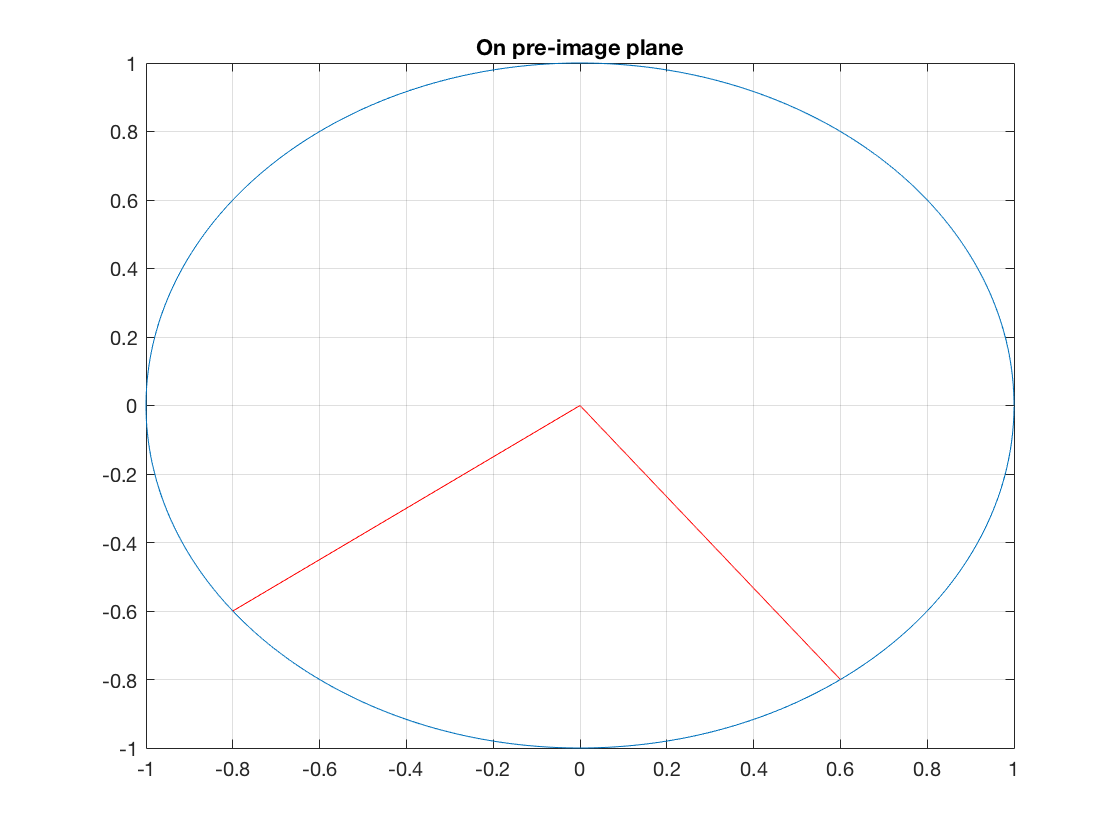
\includegraphics[scale=0.2]{pre_image}
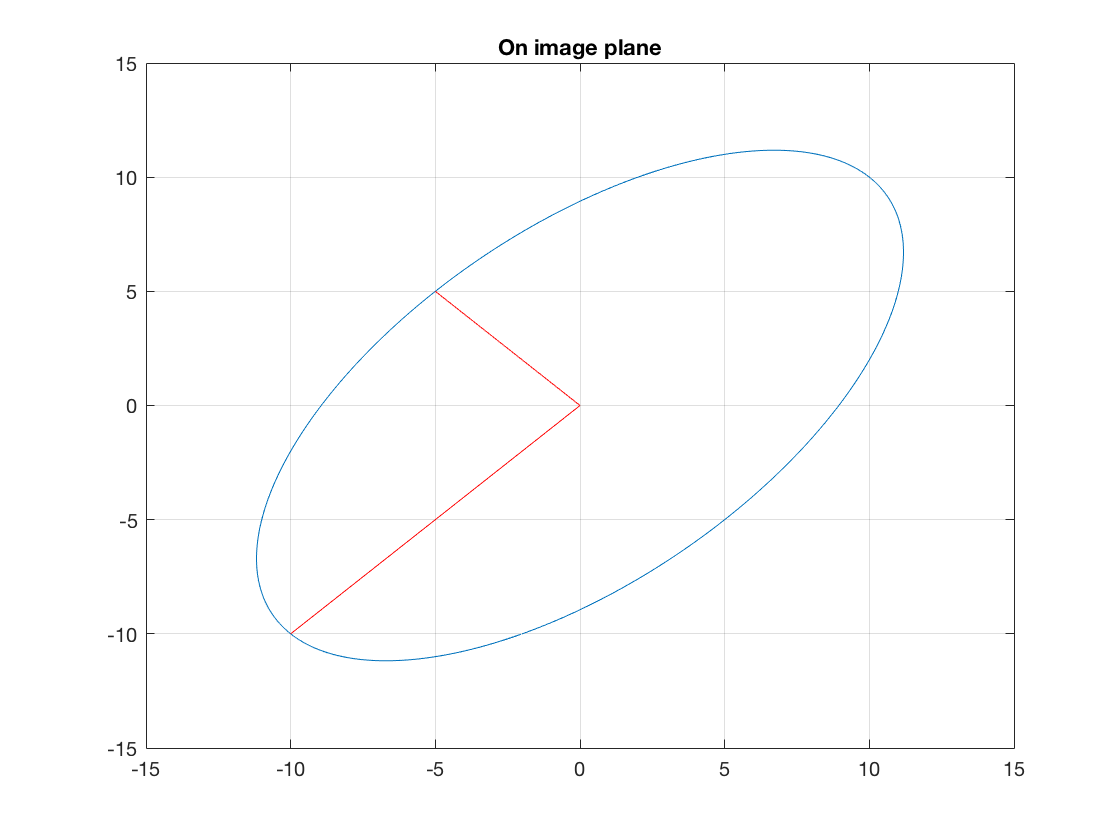
\includegraphics[scale=0.2]{image_after}
\end{figure}


\vspace{5mm}
(c)
$$\|A\|_{1}=\max_{1\leq j\leq 2} \|a_j\|_1=16.$$
$$\|A\|_{2}=\sigma_{max}(A)=10\sqrt{2}.$$
$$\|A\|_{\infty}=\max_{1\leq i\leq 2} \|a_i^{\star}\|_1=15.$$
$$\|A\|_{F}=\sqrt{\sigma_{max}^2+\sigma_{min}^2}=\sqrt{250} =5\sqrt{10}.$$

(d)
 
$$A^{-1}=(V^{\star})^{-1}\Sigma^{-1} U^{-1}=V\Sigma U^{\star}.$$
Thus, 
$$A^{-1}=\begin{bmatrix}
-\frac{3}{5}  & \frac{4}{5} \\
\frac{4}{5}  & \frac{3}{5} \\
\end{bmatrix}\begin{bmatrix}
\frac{1}{10\sqrt{2}} & 0 \\
0 & \frac{1}{5\sqrt{2}}\\
\end{bmatrix}  \frac{1}{\sqrt{2}}\begin{bmatrix}
1& 1 \\
1 & -1\\
\end{bmatrix} 
=\frac{1}{100}\begin{bmatrix}
5 &- 11 \\
10  & -2 \\
\end{bmatrix}.$$


(e) The eigenvalues of $A$ satisfies
$$ \det \left( \begin{bmatrix}
-2-\lambda & 11 \\
-10 & 5-\lambda \\
\end{bmatrix} \right) =0.$$
That is $(-2-\lambda)(5-\lambda)+110=\lambda^2+3\lambda+100=0.$

Thus $\lambda_{1,2}=\frac{1}{2}(-3\pm \sqrt{391} i )$.

(f)
$\lambda_1 \lambda_2=\frac{1}{4} (3-\sqrt{391} i)(3+\sqrt{391} i)=100.$ 
$\det(A)=-2(5)-11(-10)=100.$ 
 $\sigma_1 \sigma_2=5\sqrt{2} \cdot 10 \sqrt{2} =100.$  $ |\det(A)|=100.$
 
 (g)
 
 The area of the ellipsoid onto which $A$ maps the unit ball is  $\det(A) \cdot \mbox{ area of the unit ball in } \mathbb{R}^2=100\pi.$
\end{exercise}
\begin{exercise}
\begin{align*}
\begin{bmatrix}
0 & A^{\star} \\
A & 0 \\
\end{bmatrix} =& \begin{bmatrix}
0 & I \\
I & 0 \\
\end{bmatrix} \begin{bmatrix}
U\Sigma V^{\star}  & 0 \\
 0 & V\Sigma U^{\star} \\
\end{bmatrix} \\
{}=&  \begin{bmatrix}
0 & I \\
I & 0 \\
\end{bmatrix} \begin{bmatrix}
U  & 0 \\
 0 & V \\
\end{bmatrix} \begin{bmatrix}
\Sigma & 0 \\
0 & \Sigma \\
\end{bmatrix}
\begin{bmatrix}
V^{\star}  & 0 \\
0 & U^{\star}\\
\end{bmatrix}.
\end{align*}
Note that the inverse of  $\begin{bmatrix}
0 & I \\
I & 0 \\
\end{bmatrix} \begin{bmatrix}
U  & 0 \\
 0 & V \\
\end{bmatrix}$ is $\begin{bmatrix}
U^{\star} & 0 \\
0 & V^{\star}
\end{bmatrix} =\begin{bmatrix}
0 & I \\
I & 0 \\
\end{bmatrix} \begin{bmatrix}
V^{\star} & 0 \\
0 & U^{\star}
\end{bmatrix} .$ 
The inverse of $\begin{bmatrix}
0 & I \\
I  & 0 \\
\end{bmatrix}$ is itself.

Thus,
$\begin{bmatrix}
0 & A^{\star} \\
A & 0 \\
\end{bmatrix} =
\begin{bmatrix}
0 & I \\
I & 0 \\
\end{bmatrix} 
\begin{bmatrix}
U  & 0 \\
 0 & V \\
\end{bmatrix}\left(\begin{bmatrix}
\Sigma & 0 \\
0 & \Sigma \\
\end{bmatrix}
\begin{bmatrix}
0 & I \\
I & 0 \\
\end{bmatrix} \right) \left(\begin{bmatrix}
0 & I \\
I & 0 \\
\end{bmatrix} \begin{bmatrix}
U  & 0 \\
 0 & V \\
\end{bmatrix}\right)^{-1}.$

Note that $\begin{bmatrix}
\Sigma & 0 \\
0 & \Sigma \\
\end{bmatrix}
\begin{bmatrix}
0 & I \\
I & 0 \\
\end{bmatrix}=\begin{bmatrix}
0 & \Sigma \\
\Sigma & 0\\
\end{bmatrix}=\frac{1}{\sqrt{2}} \begin{bmatrix}
I   & I \\
I & -I \\
\end{bmatrix} \begin{bmatrix}
\Sigma  & 0 \\
0&  \Sigma \\ 
\end{bmatrix} \frac{1}{\sqrt{2}} \begin{bmatrix}
I   & I \\
I & -I \\
\end{bmatrix}.$

If $X=\frac{1}{\sqrt{2}} \begin{bmatrix}
0 & I \\
I & 0 \\
\end{bmatrix} 
\begin{bmatrix}
U  & 0 \\
 0 & V \\
\end{bmatrix} \begin{bmatrix}
I   & I \\
I & -I \\
\end{bmatrix}$, $\begin{bmatrix}
0 & A^{\star} \\
A & 0 \\
\end{bmatrix} =X \begin{bmatrix}
\Sigma & 0 \\
0 & -\Sigma \\
\end{bmatrix} X^{-1}.$
\end{exercise}


\end{document}
